\documentclass[10pt,oneside,a4paper]{book}
\usepackage[margin=2cm]{geometry}
%\usepackage{showframe}
\usepackage{graphicx}
\usepackage{parskip}
\usepackage{blindtext}
\usepackage[linktoc=all]{hyperref}
\setcounter{tocdepth}{3}
\usepackage{hyperref}
\hypersetup{colorlinks=true}
\usepackage{mathtools}
\usepackage[T1]{fontenc} 
\usepackage{lmodern}
\usepackage{listings} 
\usepackage{float}
\usepackage{makeidx}
\usepackage{minted}
\usepackage[hypcap]{caption}
\newcounter{cexctr} \setcounter{cexctr}{1}
\newcounter{pyjvexctr} \setcounter{pyjvexctr}{1}
\newcommand{\ttbf}[1]{{\ttfamily \bfseries #1}}
\newcommand{\ilCode}[1]{{\small {\ttfamily \bfseries #1}}}
\newcommand{\afuncT}[3]{\clearpage{\Large \textbf{\hypertarget{{\ttfamily \bfseries#1Func}}{#1}}{\hspace*{\fill}\hypertarget{#1Func}{}\hyperlink{#3}{up}}} \vspace{.01\textheight}\\ \hspace*{.02\textwidth} \parbox{.97\textwidth}{#2 } \vspace{.005\textheight}}
%hlinkFunk used for hyperlink of table name with function page.
\newcommand{\hlnkFunc}[1]{\hyperlink{#1Func}{\texttt{#1}}}
\newcommand{\hlnkFuncT}[2]{\hyperlink{#1Func}{\texttt{#2}}}
%
\newcommand{\cvsiplh}{ \hspace*{.02\textwidth} {\large \textbf{C VSIPL}}\vspace{.005\textheight}}
%
\newcommand{\pyjvsiph}{\hspace*{.02\textwidth} {\large \textbf{pyJvsip}}\vspace*{.005\textheight}}
% Available Functions heading
\newcommand{\afh}{\\\hspace*{.04\textwidth} \vspace*{.005\textheight}\textbf{Available Functions }}
%
\newcommand{\pyjvComment}[1]{\newline \hspace*{.02\textwidth}\textbf{Comments}\\ \hspace*{.02\textwidth}\parbox{.95\textwidth}{ \vspace*{.005\textheight}\begin{itemize}{ #1}\end{itemize}}}
%
\newcommand{\pyComment}[1]{\newline \hspace*{.04\textwidth}\textbf{Comments}\\ \hspace*{.04\textwidth}\parbox{.95\textwidth}{\vspace*{.1cm}\begin{itemize}{ #1} \end{itemize}}}
%
\newcommand{\viewmthd}[4]{\\\hspace*{.04\textwidth}\textbf{View Method}
\\ \hspace*{.06\textwidth}\textbf{Available: }#1\hspace{.25cm}\textbf{Property: }#2\hspace{.25cm}\textbf{In-Place: } #3 
\\ \hspace*{.06\textwidth}\textbf{Example:} {\ttfamily #4}}
%
\newcommand{\vmthdh}{\hspace*{.04\textwidth} \textbf{View Method}\vspace*{.005\textheight}}
%
\newcommand{\apyfunc}[2]{\newline \hspace*{.04\textwidth}\textbf{Function} 
\\ \hspace*{.06\textwidth}\textbf{Available:} #1 
\\ \hspace*{.06\textwidth}\textbf{Example:} {\ttfamily #2}}
%use as \pyjv{}
\newcommand{\pyjv}{{\ttbf{pyJvsip}}}
%use as \jv{}
\newcommand{\jv}{\ttbf{JVSIP}}
%use as \cvl{}
\newcommand{\cvl}{\ttbf{C VSIPL}}
% from http://mirrors.rit.edu/CTAN/info/digests/ttn/ttn2n3.pdf
\newcommand\Ts{\rule{0pt}{2.6ex}}
\newcommand\Bs{\rule[-1.2ex]{0pt}{0pt}}
\makeindex
\begin{document}
\afuncT{clip}{Clip. Computes the generalized double clip of two views. See \cvl{} specification for more information.}{selectionOperations}
\\\cvsiplh
\afh
{
\ttfamily
\\\hspace*{.04\textwidth}\begin{tabular}[H]{l}
void vsip\_mclip\_d(\\*\hspace*{1cm}const vsip\_mview\_d*, vsip\_scalar\_d, vsip\_scalar\_d,\\*\hspace*{1cm}vsip\_scalar\_d, vsip\_scalar\_d, const vsip\_mview\_d*);\\
void vsip\_mclip\_f(\\*\hspace*{1cm}const vsip\_mview\_f*, vsip\_scalar\_f, vsip\_scalar\_f,\\*\hspace*{1cm}vsip\_scalar\_f, vsip\_scalar\_f, const vsip\_mview\_f*);\\
void vsip\_mclip\_i(\\*\hspace*{1cm}const vsip\_mview\_i*, vsip\_scalar\_i, vsip\_scalar\_i,\\*\hspace*{1cm}vsip\_scalar\_i, vsip\_scalar\_i, const vsip\_mview\_i*);\\
void vsip\_mclip\_si(\\*\hspace*{1cm}const vsip\_mview\_si*, vsip\_scalar\_si, vsip\_scalar\_si,\\*\hspace*{1cm}vsip\_scalar\_si, vsip\_scalar\_si, const vsip\_mview\_si*);\\
void vsip\_vclip\_d(\\*\hspace*{1cm}const vsip\_vview\_d*, vsip\_scalar\_d, vsip\_scalar\_d,\\*\hspace*{1cm}vsip\_scalar\_d, vsip\_scalar\_d, const vsip\_vview\_d*);\\
void vsip\_vclip\_f(\\*\hspace*{1cm}const vsip\_vview\_f*, vsip\_scalar\_f, vsip\_scalar\_f,\\*\hspace*{1cm}vsip\_scalar\_f, vsip\_scalar\_f, const vsip\_vview\_f*);\\
void vsip\_vclip\_i(\\*\hspace*{1cm}const vsip\_vview\_i*, vsip\_scalar\_i, vsip\_scalar\_i,\\*\hspace*{1cm}vsip\_scalar\_i, vsip\_scalar\_i, const vsip\_vview\_i*);\\
void vsip\_vclip\_si(\\*\hspace*{1cm}const vsip\_vview\_si*, vsip\_scalar\_si, vsip\_scalar\_si,\\*\hspace*{1cm}vsip\_scalar\_si, vsip\_scalar\_si, const vsip\_vview\_si*);\\
void vsip\_vclip\_uc(\\*\hspace*{1cm}const vsip\_vview\_uc*, vsip\_scalar\_uc, vsip\_scalar\_uc,\\*\hspace*{1cm}vsip\_scalar\_uc, vsip\_scalar\_uc, const vsip\_vview\_uc*);\\
\end{tabular}
}
%
\\\pyjvsiph
\viewmthd{No}{NA}{NA}{NA}
%
\apyfunc{Yes}{\ttbf{clip(in,t1,t2,c1,c2,out)}}
\inputminted[linenos=true,resetmargins=true,xleftmargin=.12\textwidth,fontfamily=tt,fontsize=\small]{python}{./pyJvsip_examples/eXclip.py}
\hspace*{.08\textwidth}{\rmfamily For result see figure \ref{fig:ClipExample}.}\\
\begin{minipage}[c]{\textwidth}\centering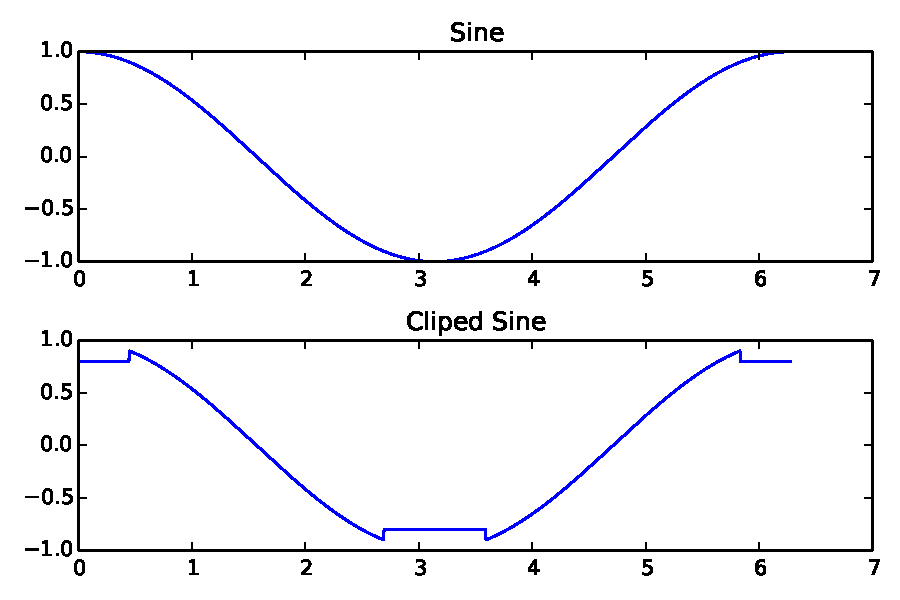
\includegraphics[width=0.8\textwidth]{./pyJvsip_examples/eXclip}\captionof{figure}{Clip Example}
\label{fig:ClipExample}\end{minipage}
\pyComment{
\item{The clip function works much the same as \cvl{} except the output is returned. In line 6 of the example we used the \ttbf{empty} method to create the output vector and saved a reference in the left value.}
\item{The \ttbf{clip} function is a bit complicated. See the \cvl{} specification for more complete details.}
\item{The \ttbf{view} \ttbf{in} is clipped according to the rules of the function. The clipping checks are set by \ttbf{t1} and \ttbf{t2} and the clip values are set by \ttbf{c1} and \ttbf{c2} accordingly. The output is placed in \ttbf{out}. If \ttbf{in==out} then the function is done in-place}
}
\end{document}